\documentclass[a0paper,portrait]{baposter}

\usepackage{wrapfig}
\usepackage{lmodern}
\usepackage{amsmath}
\usepackage{enumitem}
\usepackage{xcolor}
\usepackage{caption}

\usepackage[utf8]{inputenc} %unicode support
\usepackage[T1]{fontenc}

\usepackage{hyperref}

\selectcolormodel{cmyk}

\graphicspath{{figures/}} % Directory in which figures are stored


\newcommand{\compresslist}{%
\setlength{\itemsep}{0pt}%
\setlength{\parskip}{1pt}%
\setlength{\parsep}{0pt}%
}

\newenvironment{boenumerate}
  {\begin{enumerate}\renewcommand\labelenumi{\textbf\theenumi.}}
  {\end{enumerate}}



\begin{document}

\definecolor{darkblue}{rgb}{0.1,0.2,1.0}
\definecolor{lightblue}{rgb}{0.2,0.4,0.8}

\begin{poster}
{
grid=false,
headerborder=open, % Adds a border around the header of content boxes
colspacing=1em, % Column spacing
bgColorOne=white, % Background color for the gradient on the left side of the poster
bgColorTwo=white, % Background color for the gradient on the right side of the poster
borderColor=darkblue, % Border color
headerColorOne=lightblue, % Background color for the header in the content boxes (left side)
headerColorTwo=lightblue, % Background color for the header in the content boxes (right side)
headerFontColor=white, % Text color for the header text in the content boxes
boxColorOne=white, % Background color of the content boxes
textborder=rounded, %rectangle, % Format of the border around content boxes, can be: none, bars, coils, triangles, rectangle, rounded, roundedsmall, roundedright or faded
eyecatcher=false, % Set to false for ignoring the left logo in the title and move the title left
headerheight=0.11\textheight, % Height of the header
headershape=rounded, % Specify the rounded corner in the content box headers, can be: rectangle, small-rounded, roundedright, roundedleft or rounded
headershade=plain,
headerfont=\Large\textsf, % Large, bold and sans serif font in the headers of content boxes
%textfont={\setlength{\parindent}{1.5em}}, % Uncomment for paragraph indentation
linewidth=2pt % Width of the border lines around content boxes
}
{}
%
%----------------------------------------------------------------------------------------
%	TITLE AND AUTHOR NAME
%----------------------------------------------------------------------------------------
%
{
\textsf %Sans Serif
{Evaluation of different techniques for image augmentation.
}
}
{\sf\vspace{0.5em}\\
Ralph Lesch and Joshua Heipel
\vspace{0.1em}\\
\small{University of Freiburg, Department of Computer Science, Deep Learning Bachelor Project
\vspace{0.2em}\\
ralph.lesch@neptun.uni-freiburg.de  ,  joshua.heipel@gmx.de}
}
%{
\includegraphics{logo}} % University/lab logo


\headerbox{1. Introduction}{name=introduction,column=0,row=0, span=3}{
Convolutional Neural Networks (CNNs) have become a major aproach for the task of Semantic Segmentation and are nowadays used widely over many different fields of applications. Although for some use cases large datasets with thousands of (manually) labeled images have been published (such as CamVid or CityScape in the context of city traffic), in many situations appropriate training data still remains sparse. As a consequence Deep Neural Networks with lots of trainable parameters tend to overfit small and monotonous datasets while generating poor predictions for new (unseen) observations. In order to improve generalization of such CNNs existing training data can be extended by employing different techniques of image augmentation. 
\vspace{5px}
}


\headerbox{2. Architecture}{name=architecture,column=0,below=introduction,span=1}{


In our case study we use a hierarchical encoder-decoder network with skip connections (CNN of exercise 3) to compare different settings:

\begin{enumerate}[label={(\arabic*)}]
    \item \textbf{No Augmentation}
    \item \textbf{Shape Augmentation} by applying different geometric transformation and dropouts (Horizontal Flip, Scaling, Crop and Padding, rectangular Cutouts)
    \item \textbf{Color Augmentation} by varying the intensity values (Adjustment of Brightness and Contrast, Color shifts)
    \item \textbf{Shape \& Color Augmentation}
\end{enumerate}
\vspace{13px}
}



\headerbox{3. Training}{name=training,column=0,below=architecture,span=1}{

The network is trained on the CamVid dataset which contains 7707 (manually) labeled images. To allow for a fair comparison between our different configurations (1) - (4), we use the same hyperparameters (namely the total amount of iterations and batch size) for all types of augmentations. Batches are created by sampling images from the original dataset with pseudo-random numbers and then applying augmentations for setting (2) - (4) on 90\% of the images. In order to investigate the effect of applying augmentation on sparse data we train the network (I) on the full dataset and (II) with a small subset of 468 images.

\begin{center}
    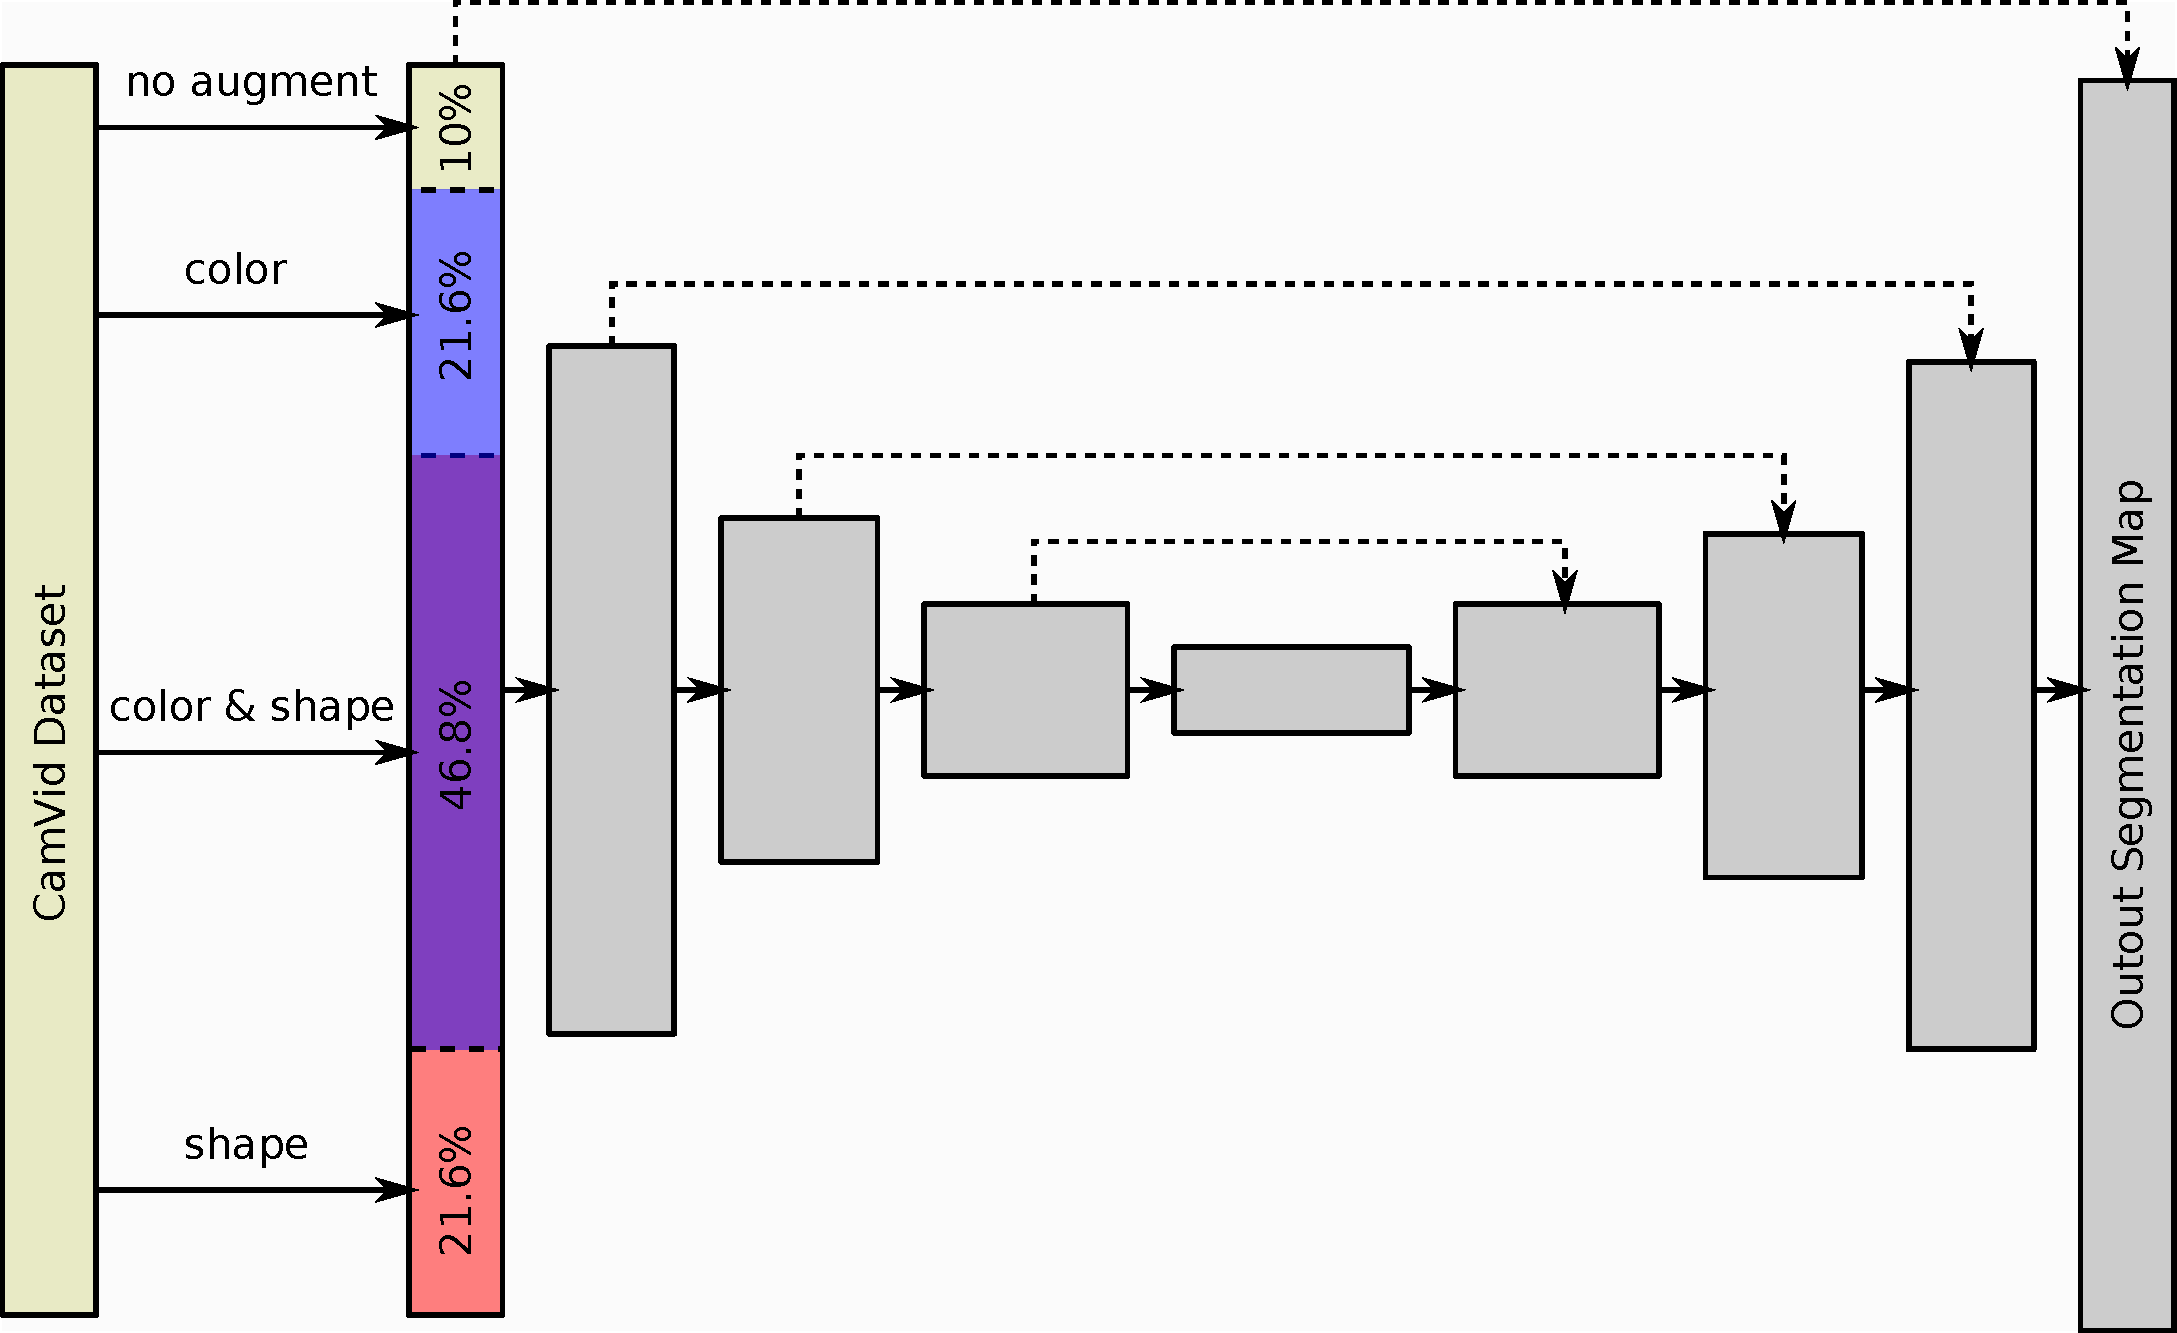
\includegraphics[width=0.9\linewidth]{cnn.pdf}
    \captionof{figure}{Configuration (4) with shape \& color augmentations.  90\% of all images are randomly modified and fed into the encoder-decoder network with skip connections.}
\end{center}
\vspace{13px}
}


\headerbox{4. Examples}{name=examples,span=2,column=1,below=introduction}{ 

\begin{wrapfigure}{l}{0.45\textwidth}
    \begin{center}
        \includegraphics[width=0.8\linewidth]{augmentation.pdf}
        \caption{Different types of augmentations. From left: original image,  original segmentation map, augmented image and augmented segmentation map.}
    \end{center}
\end{wrapfigure}

To facilitate multiple independent modifications $A_k$ (e.g. cropping and flipping an image) we implemented our own probabilistic framework based on the principle of inclusion and exclusion, where:
%\[P(A_i \cup A_j) = P(A_i) + P(A_j) - P(A_i \cap A_j)\] \[= 2\cdot P(A_i) - P(A_i)^2\] or in more general form: 
\[P\left(\bigcup_{k=1}^{n} A_k\right) = \sum_{k=1}^{n} (-1)^{(k+1)} \begin{pmatrix} n \\ k \\\end{pmatrix}P(A_k)^k,\]
which randomly selects different types of augmentations in varying order. We use the same probability for shape or color modification when investigating setting (4). Because of storage limitations all augmentations are calculated \textit{"on the fly"} using {\color{darkblue} Python 3.5} together with {\color{darkblue} Numpy}, {\color{darkblue} Scipy} and the {\color{darkblue} Imgaug} package, before feeding the batches into the CNN.
In order to parametrize shape and color modifications we draw samples from uniform distribution. Upper and lower bounds are adjusted by manually applying augmentations on different images of the CamVid dataset. The range of possible modifications is thereby limited to realistic variations that correspond to natural changes of lightning conditions and scale transformations. Cutout and padding modifications are chosen to cover at most 1/10 resp. 1/3 of all pixels.

\vspace{10px}

}


\headerbox{5. Results}{name=results,span=2,column=1,below=examples}{ 

\begin{minipage}[t]{0.49\textwidth}\centering
    \vspace{0pt}
    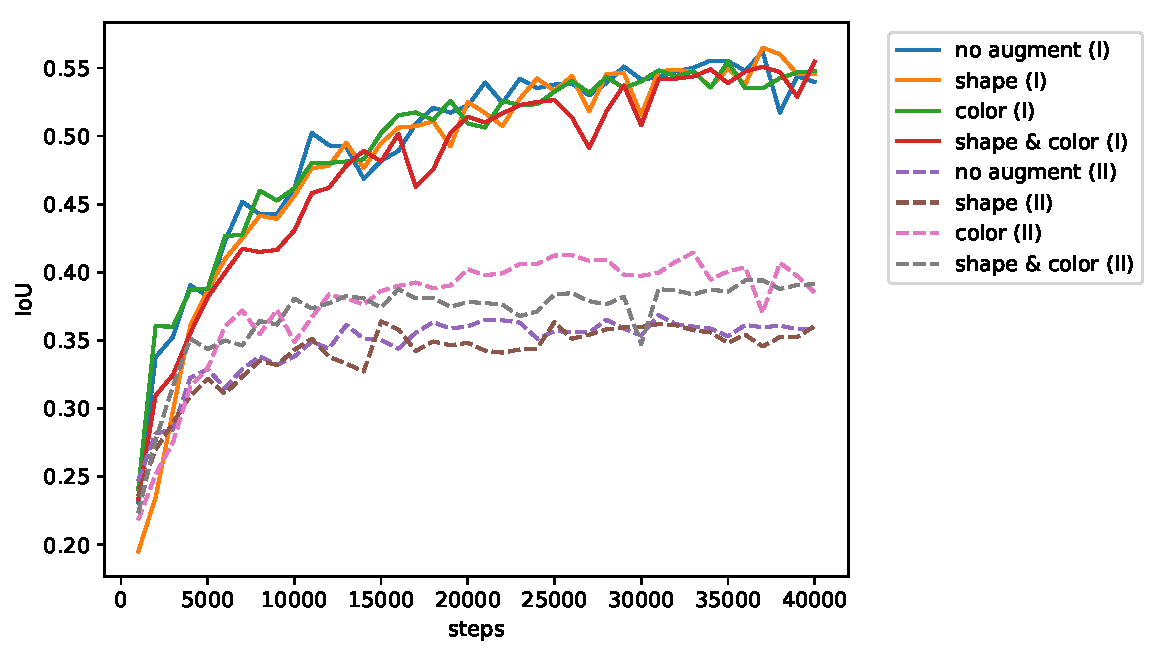
\includegraphics[width=\linewidth, keepaspectratio,trim={0 10px 0 0}, clip]{result.pdf}
    \captionof{figure}{Learning curves with the Intersections over Union (IoU) of both large (I) and small (II) dataset with configurations (1) - (4).}
\end{minipage}\hfill
\begin{minipage}[t]{0.49\textwidth}\centering
    \vspace{4pt}
    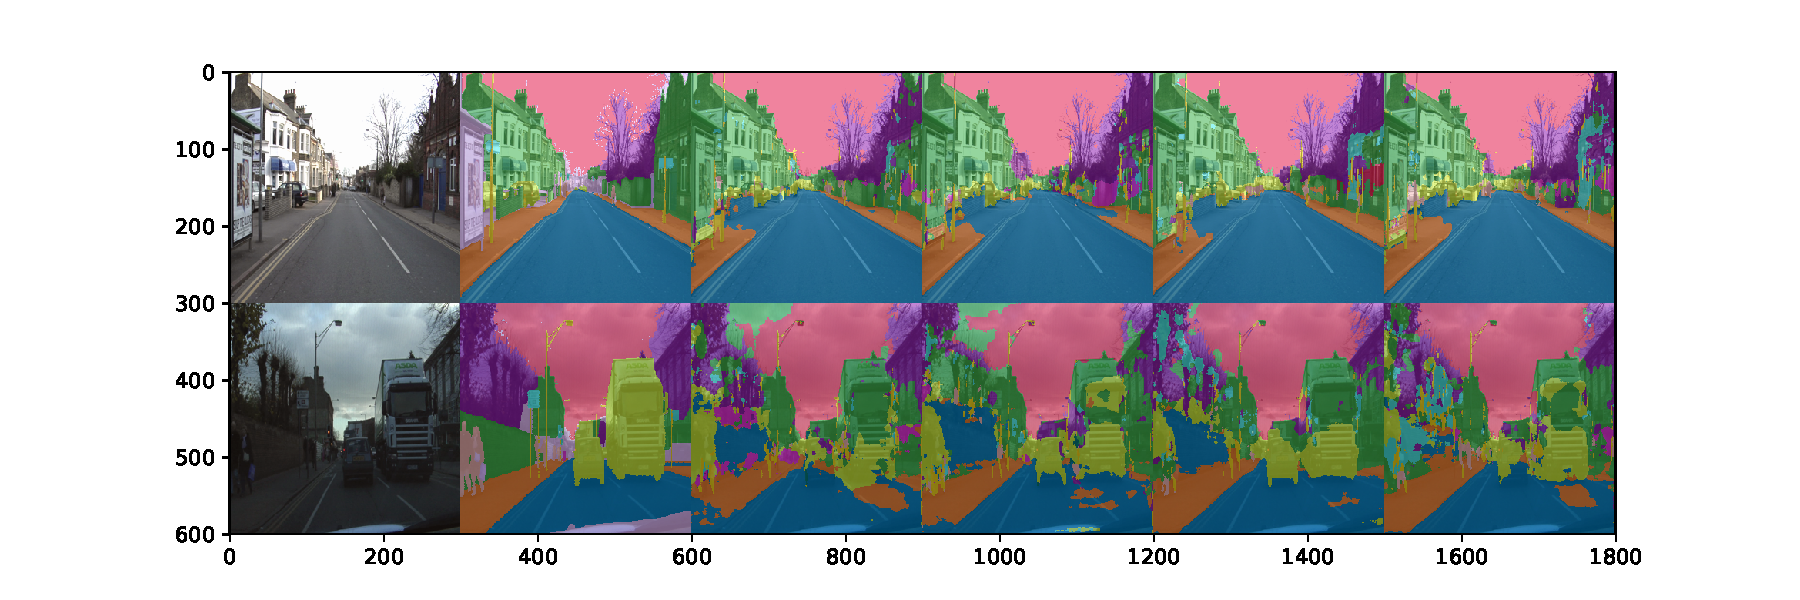
\includegraphics[width=\linewidth]{prediction.pdf}
    \captionof{figure}{Images and predicted segmentation maps for the test data. From left: original image and segmentation map, predictions without augmentation, with shape, color, shape \& color augmentations.}
\end{minipage}
\vspace{.5\baselineskip}

We observe a different performance of the network for configurations (1) - (4) when trained either on the small or on the full dataset. If a large amount of data is available (I), the learning curves show similar trajectories. With sparse training data (II) randomly applied augmentations have a positive effect on the quality of network predictions. Here we see the color augmentation (3) clearly outperform the shape augmentation (2), which gives no clear improvement.\\
However the gain in performance is not enough to achieve results that are as accurate as with a larger and more variable dataset.
\vspace{10px}
}


\headerbox{6. Conclusions}{name=conclusion,column=0,below=training,span=2,above=bottom}{

\begin{itemize}
    \item Random modifications applied on sparse datasets can improve performance of CNNs.
    \item Color augmentation (3) results in a better performance than shape augmentation (2).
    \item Parameters for different augmentations must be chosen carefully to have the best positive effects and might be optimized with hyperparameter optimization methods.
\end{itemize}

}


\headerbox{7. References}{name=references,column=2,span=1,below=results,above=bottom}{

%\small % Reduce the font size in this block
\renewcommand{\section}[2]{\vskip 0.05em} % Get rid of the default "References" section title
%\nocite{*} % Insert publications even if they are not cited in the poster

\begin{itemize}
    \item Source:\\ github.com/RalphLesch/dl-lab-2018-project
    \item Network based on exercise3\_CV\_ML:\\ github.com/aisrobots/dl-lab-2018
\end{itemize}

%\bibliographystyle{unsrt}
%\bibliography{poster} % Use sample.bib as the bibliography file
}

\end{poster}

\end{document}
